\section {Interfacing to the outside world}
\index {Interfacing to the outside world}

Here we deal with the basic principles of getting the WebBrick to control and listen to the outside world.

\subsection {Basics}

The WebBrick treats the Digital Inputs as push to make inputs.  There is a software option that can allow
the use on off switches.

To action, the push button should ground the input, pullups are enabled at the PIC chip.  
In out test applications we use CAT5e cable and have runs of up to 100m between the WebBrick 
and the switches, use a twisted pair for each input to reduce noise pickup.  We have seen 
pickup cause problems, in our case we grounded unused cores which cured the issues.

The outputs at Digital Output Low (DOL) are TTL and should be treated as such, they have enough current 
sourcing to drive two LEDs and a Solid State Relay.  In our test applications we drive 
one LED and an SSR simultaneously.

The outputs at Digital Output High (DOH) are open collector capable of sinking 500mA, this means 
the device being switched is connected to a supply rail and the outputs go low on activation to 
switch on the device. Do not use more than 12v as the supply to the device.

The monitor inputs have no pullups are very sensitive, so if not connected to anything or 
connected to a source that does not actively drive high or low tie down to 0V with a 4.7K resistor. 
Valid input range is 0-5V

The analogue outputs are buffered and provide a 0-10V output good enough to drive a pair of LEDs. 
The User interface is
calibrated as 0-100\% so 10\% corresponds to 1V unless some other signal conditioning is inserted.
Do NOT try to drive an LED and an opto isolator at the same time, the forward drop on the LED's will 
be different and the results not much fun (you could use separate resistors to drive each).

\subsection{Cabling}
\index{Cabling}

The webBrick has been designed to use standard CAT 5 networking or structured cabling. CAT 5 cable has consists of 
4 pairs of wires in a single sheath.
These are colour coded with the first colour being the main colour and the later being just narrow stripes:

    \begin{itemize}
			\item Brown with White and White with Brown. 
			\item Green with White and White with Green. 
			\item Orange with White and White with Orange. 
			\item Blue with White and White with Blue. 
    \end{itemize}

To reduce any possible interference the pairs should be used properly with a pair for each 
input or output. Even when multiple inputs are run on the same cable do not use a single ground wire and multiple
input wires, use a ground wire for each input wire. Similarly for outputs.



\subsection{Digital Inputs}

	\subsubsection{Digital Input Characteristics}
	\index{Digital Input Characteristics}
	
		Before looking at the components that can be connected to a WebBrick is useful to look at the timing and voltage characteristics
		of the Digital inputs:
		
		    \begin{figure}[H]
		    \centering
		    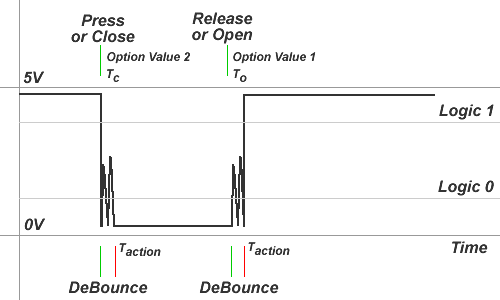
\includegraphics[width=0.5\textwidth]{Images/DigitalInChar.png}
		    \end{figure}
		    
		The diagram shows an example of a simple pushbutton connected between a Digital Input and WebBrick Ground.
		
		Whilst the button is open, the voltage on the Digital Input will measure near 5V (typically 4.9). When the button
		is pressed this will fall to zero or near zero (anything below 0.6V is considered zero).
		
		Note that in the diagram we have represented some switch bounce. \index{Digital Input DeBounce} The WebBrick has internal
		debouncing of around 20mS.
		
		Because the WebBrick is designed to be used with a range of input devices, it has an option that sets when the state engine
		get triggered:
		
			\begin{description}
				\item[{\bf Rising Edge}] Option is set to 1
				\item[{\bf Falling Edge}] Option is set to 2 - this is the default behaviour
				\item[{\bf Both Edges}] Option is set to 3
			\end{description}
		
		    \begin{figure}[H]
		    \centering
		    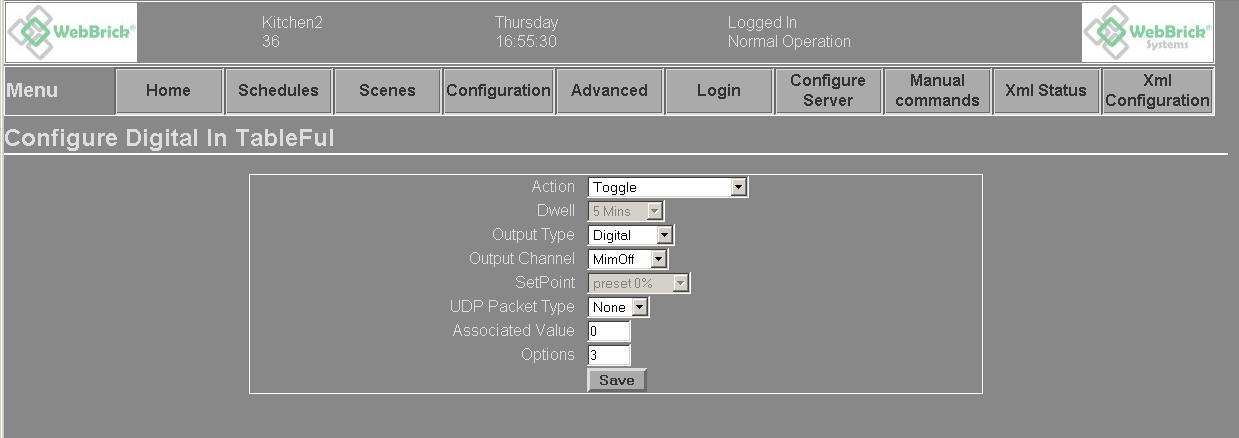
\includegraphics[width=0.5\textwidth]{Images/DigitalIn.png}
		    \end{figure}


	\subsubsection{Switches}
	For real use, we've found that push buttons with integral LEDs not only look good, but can be very practical.

	A background glow is helpful for locating the button in the dark.

	We either use a 10K resistor to provide a 'background' glow for the 'Off' condition and a 330ohm or 1k resistor 
	from the corresponding digital output to confirm the 'On' condition.

	{\it Note} \index{using 'MK' style switches} It is quite possible to use simple toggle switches with the WebBrick.  However it
	is likely that you'll want to trigger the state engine on both the 'close' and 'open' action.  In this case the option value should
	be set to '3'.  See the section on Digital Input Characteristics for more detail.

	\subsubsection{PIR Passive Infra Red sensors}
	\index{PIR Passive Infra Red sensors}
	These typically have a dry contact that closes for a period of time on detection of movement and can be
	connected to a WebBrick input.

	\subsubsection{Light sensor}
	\index{Light sensor}
	These can also be connected to a digital input unless you have a type that provides a voltage dependant on
	the light level then it should be connected to an analogue input.

	\subsubsection{Security switches}
	\index{Security switches}
	Magnetic reed relays for door and window detection. These are typically used for burglar alarms but can just as easily be
	used to connect to WebBricks.

	\subsection{Digital Outputs}

	\subsubsection{Driving LEDs}
	\index{LEDs ! Driving}

	LEDs are now affordable for just about every kind of use and available in all sorts of colours and power.  
	Therefore its worth a section here describing how they can be used with the WebBrick.

	For simple indication purposes a 300R resistor in series with the TTL level digital outputs will give 
	sufficient current for a standard 3/5mm LED.  There is still sufficient drive to operate solid state 
	relays. \index{SSRs}

	\subsection{Open Collector Outputs}
	\index{Open Collector Outputs}
	
		These can sink up 500mA on a channel with a limit of 800mA across all 8 outputs at any one time.

		We have also found that modern high brightness white LEDs make very good night lighting that can be switched from
		a WebBrick using the Open collector driver.

	\subsubsection{Solid state relays}

	We've been using the Crydom EZ240D5 solid state relays to great effect.  These can be connected directly to 
	the Digital outputs with no other components.

	\subsection{Analogue Inputs}

		These can be used to interface anything that provides a 0-5V output or can be set to produce a 0-5V input. 
		You could also connect an ordinary potentiometer to this input. You should not exceed 5V but higher voltages 
		could be reduced using a two resistor potential divider.

	\subsection{Analogue Outputs}

	\subsubsection{Dimmers}
	\index{Dimmers}

	Any dimmer that accepts a 0-10V control signal can be connected to the analogue outputs.

	We have used the Velleman K8003 kits now replaced by the K8064.

	CPC have some 4 channel dimmers.
	\begin{verbatim}http://cpc.farnell.com/jsp/endecaSearch/partDetail.jsp?SKU=DP26289&N=411\end{verbatim}
	\begin{verbatim}http://cpc.farnell.com/jsp/endecaSearch/partDetail.jsp?SKU=DP27530&N=411\end{verbatim}

	\subsection{Mains Outputs}
	\index{Mains Outputs}

		These are zero voltage switched triacs and can handle loads up to 500W, with a total of 1500W across all 4. 
		They should be able to drive all types of load. Note that there is an internal 6.3A fuse. \index{Internal Fuse}

	\subsection{Relay Outputs}
	\index{Relay Outputs}
	
		These are double pole changeover relays. Particularly useful for curtain motors and other drapery controls. 

	\subsection{Rotary encoder}
	\index{Rotary encoder}

		This is a 3 wire device with a common connection and two signal wires. It is connected to an even/odd pair
of digital inputs with the even trigger definition controlling the action when turned one way and the odd trigger 
defintion the action when turned the other way, i.e. up/down. The target is typically one of the analogue output 
or next/prev scene. It is possible to configure some weird actions like one way is brighter and the other way is off.

	\subsection{Using Temperature Sensors}
	\subsection{Temperature Sensors}


	Here we deal with the basic principles of using the temperature sensors.

	\subsubsection{Hardware}

	The temperature sensors are accessed using the DALLAS one wire interface protocol with the master
	functionality handled by the PIC chip. The Webbrick6 supports up to 5 DS18B20 temperature sensors. 
	These sensors have a 64 bit address that 
	can be used to uniquely identify them and they can read to a resolution below 0.1 degrees C.

	\subsubsection{Software}

	Every second, an attempt is made to read the temperature from one of the sensors and update 
	the status and values. At start up and on command (RT manual command) the bus will be scanned for new devices. 
	When a new sensor is found it is read to see whether it has been tagged previously, if it 
	is untagged or the tag corresponds to a currently active sensor then a new tag number is 
	generated and stored within the sensor. When a web brick is switched on these tags 
	keep the sensors in the same order within the temperature table. The values are all 
	available in the status XML. [NOTE this will change now we have room to store the device
	addresses in the WebBrick]

	When a successful reading is taken it is recorded. Temperature sensor 1 will be tested 
	against the Low and High trigger threshold. If the value is outside these values then 
	the relevant triggers are processed, these are identical to the digital input trigger configuration.

	% COMMENTED OUT
	%\subsection {Practical Application}

	%In the real world, where you measure the temperature and where you action the results are 
	%often not the same place.

	%This is easy to achieve if you have two WebBricks.  You can arrange for one WebBrick to 
	%be near where you need to 
	%measure temperature and the second, say, in a boiler room.

	%The first WebBrick would be configured to trigger a Digital Input channel that was itself configured to generate 
	%a remote command.  This remote command would be directed at the second WebBrick.  The second WebBrick would then 
	%control the boiler.

	%This allows for a network of WebBricks that could all send commands to the 'Boiler WebBrick'.  This would then 
	%give a fine degree of control since each WebBrick could have its 'Context' changed to control behaviour, so 
	%individual zones could be configured by time to suppress requests to the Boiler WebBrick.  For 'vacation' 
	%mode, the Boiler WebBrick could have its 'Context' set to 'Commands Disabled' so that it would turn off 
	%the Boiler and not action any requests from the other WebBricks.

	\subsubsection{Installing}
	So as to get sensors to display in your desired order in the list of temperatures. You should connect them one at a time
	with the first sensor getting tagged to display in 1st row and each subsequent being in subsequent rows.
	After connecting a sensor issue manual command RT and wait for each it to register before adding the next sensor.
